\chapter{Dataset Preparation}

 \begin{figure*}[htbp]
    \centering
    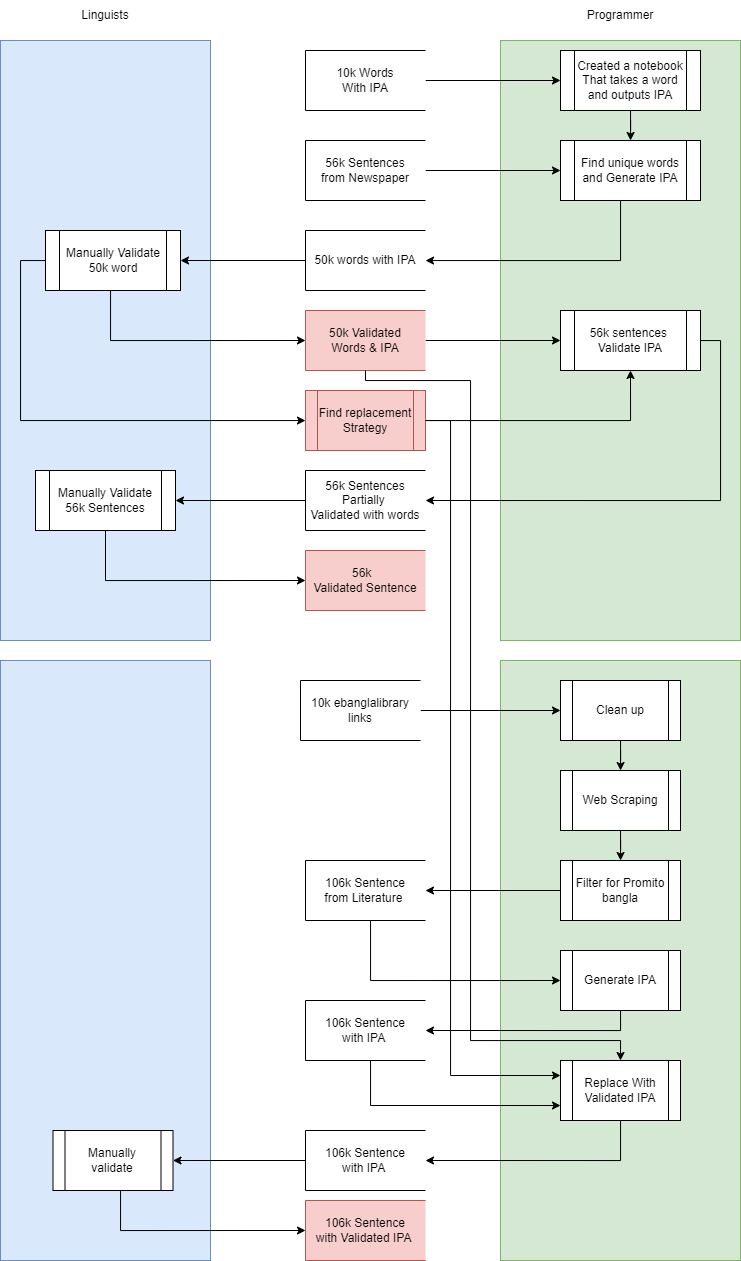
\includegraphics[scale=0.35]{Images/Diagram/preparation.png}
    \caption{Dataset Preparation Steps}
    \label{fig:preparation}
\end{figure*} 


Here we're going to describe the rigorous process of preparing the DUAL-IPA dataset step by step, explaining the whole process end to end which is shown above in the Figure \ref{fig:preparation}.
\section{Data Collection}
\subsection{Sourcing a Diverse Corpus}
\begin{itemize}
    \item The Journey began with identifying suitable sources for Promito Bangla words and sentences.
    \item Meticulously selected two distinct domains as shown in the figure \ref{fig:Sentence sources}:

        \begin{figure}[h!]
            \centering
            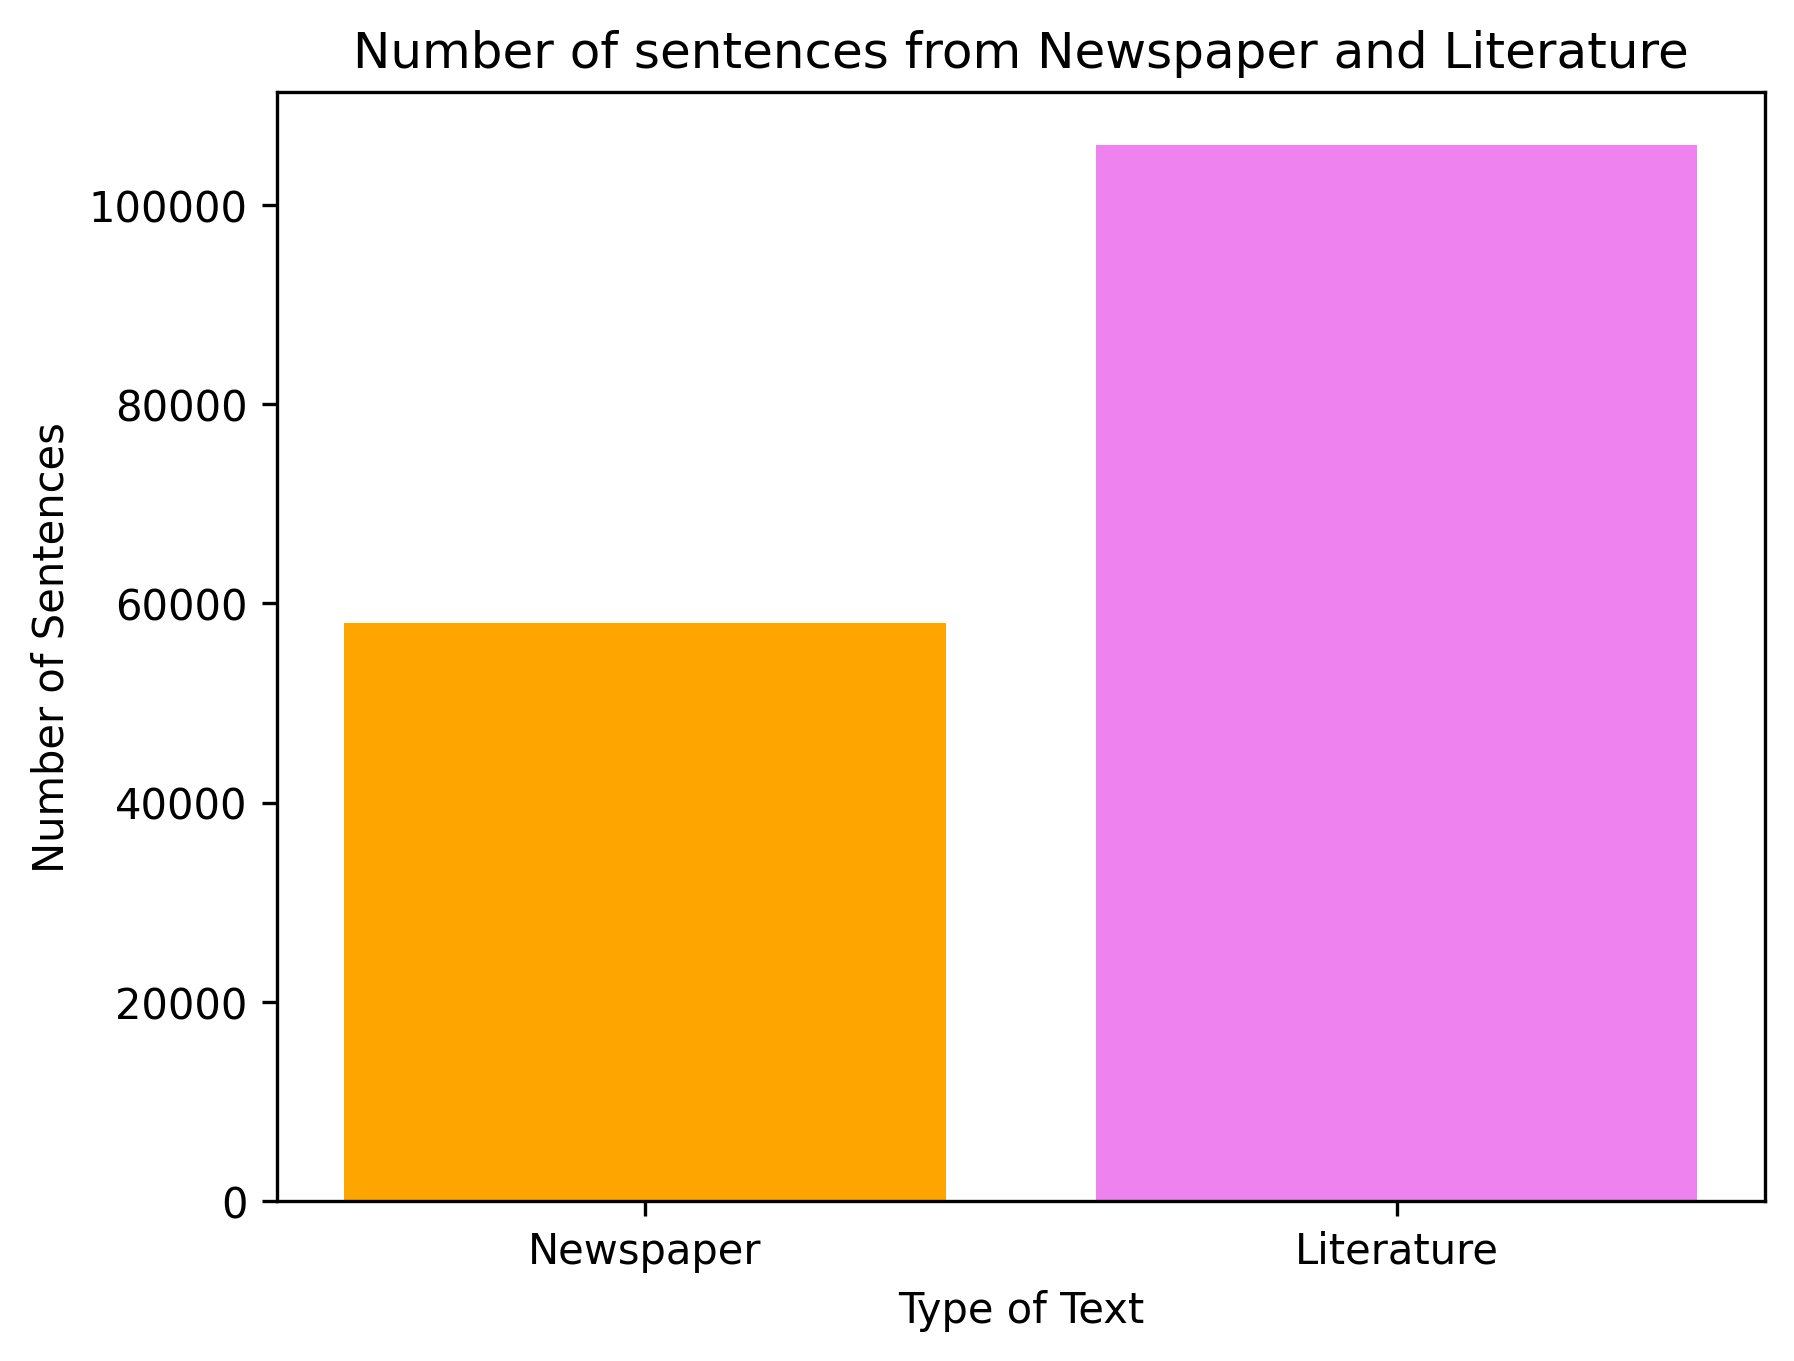
\includegraphics[scale=1]{Images/Graph/output.png}
                \caption{Sentence sources}
            \label{fig:Sentence sources}
        \end{figure}

    
    \begin{itemize}
        \item \textbf{Newspapers (33\%):} Online news articles capturing contemporary Bangla words with diverse vocabulary, which was provided to us by Bengali.AI.
        \item \textbf{Literature/Books (66\%):} Scraped novels, poems, stories and published works from \href{https://www.ebanglalibrary.com/}{Ebangla Library}  to capture nuanced beauty and historical richness.
    \end{itemize}
    \item The Balanced approach ensures that the dataset encompasses both dynamic daily communication and the enduring essence of Bangla literature.
\end{itemize}


\subsection{Quantity}
In total, 162k+ data were curated for the DUAL-IPA dataset.
\begin{itemize}
    \item \textbf{Words:} In total, almost 50k unique words were curated from the 56k sentences that are from newspapers, which were provided by Bengali.AI.
    \item \textbf{Sentences:} Total 162k sentences were curated for the dataset from newspaper and literature combined, which was scraped and curated by us. Here is the process.
    \begin{itemize}
        \item We were given a list consisting of, 10993 unique Ebangla Library links.
        \item We removed the non-promito from the list. Then we had 9971 links. Then we had 9971 links. The links contained sentences from \textbengali{"রমণীমোহন মল্লিক","শ্রীকৃষ্ণকীর্তন", "বাংলা বেদ - ঋগ্বেদ সংহিতা", "বাংলা হাদিস", "বাংলা মহাভারত",  "বাংলা রামায়ণ", "গীতা-প্রসঙ্গ", "বাংলা গীতা", "ঈশ্বরচন্দ্র বিদ্যাসাগর", "কমলকুমার মজুমদার", "কাব্যগ্রন্থ", "গীতিগ্রন্থ", "বোদলেয়ার: তাঁর কবিতা", "মাইকেল মধুসূদন দত্ত - চতুর্দশপদী কবিতাবলী", "মাইকেল মধুসূদন দত্ত - মেঘনাদবধ কাব্য", "রাজশেখখর বসুর কবিতা", "হিন্দুধর্ম", "হুমায়ুন আজাদ - কাব্যসংগ্রহ", "শামসুর রাহমান - কাব্যগ্রন্থ","রুদ্র মুহম্মদ শহিদুল্লাহ - কাব্যসংগ্রহ","কবিতাবলী"} etc.
        \item We created a simple web scrapper to collect the sentences from the links.
        \item We collected 120k sentences, but these contained non-promito words. In total, we collected, 106494 unique sentences from Bangla literature.
    \end{itemize}
\end{itemize}

\subsection{Diversity}
To make sure the data doesn't represent a particular type or group of words, we made sure to source our data from multiple categories of literature categories and newspapers that represent our daily communication usage and also get the essence of the rich literature history we have in Bangla. \\
\hspace{0.5cm}This dataset contains different lengths of words in the sentences that have been curated. From 1 to 17 character is present in words. The statistics are shown below in the figures.
        \begin{figure}[h!]
            \centering
        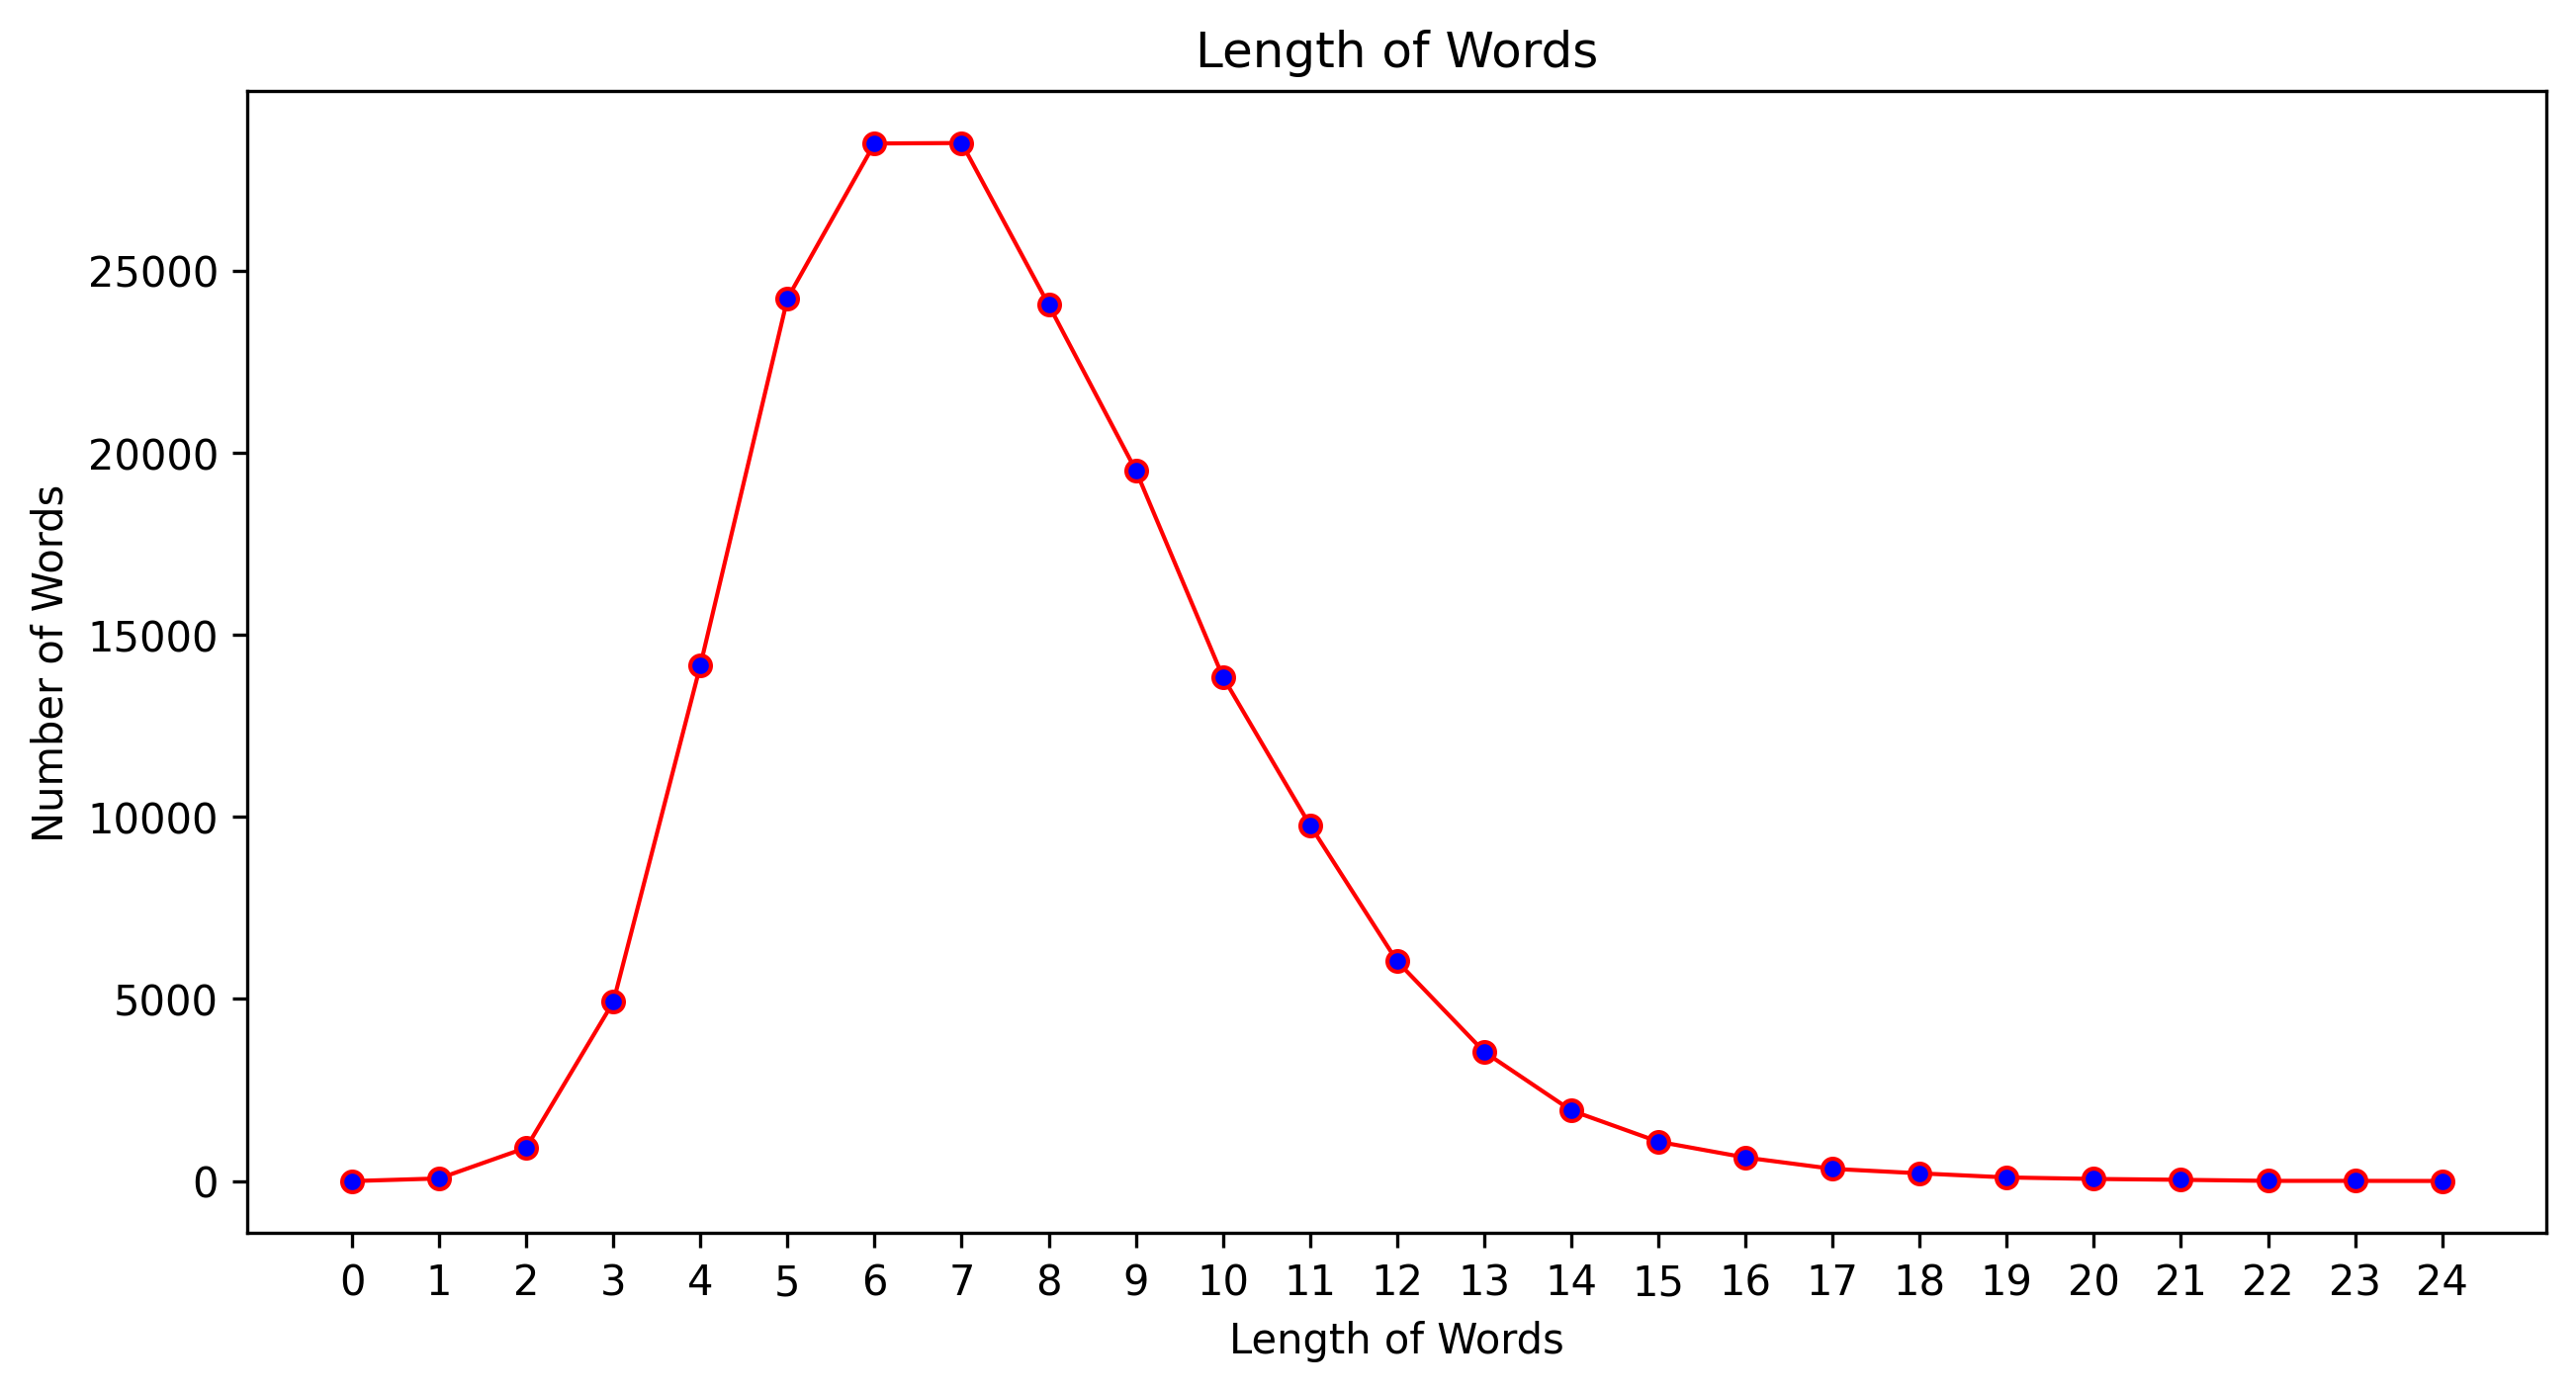
\includegraphics[scale=.7]{Images/Graph/output2.png}
                \caption{Length of words}
            \label{fig: Length of words}
        \end{figure}
        \newpage        
        \begin{figure}[h!]
            \centering
        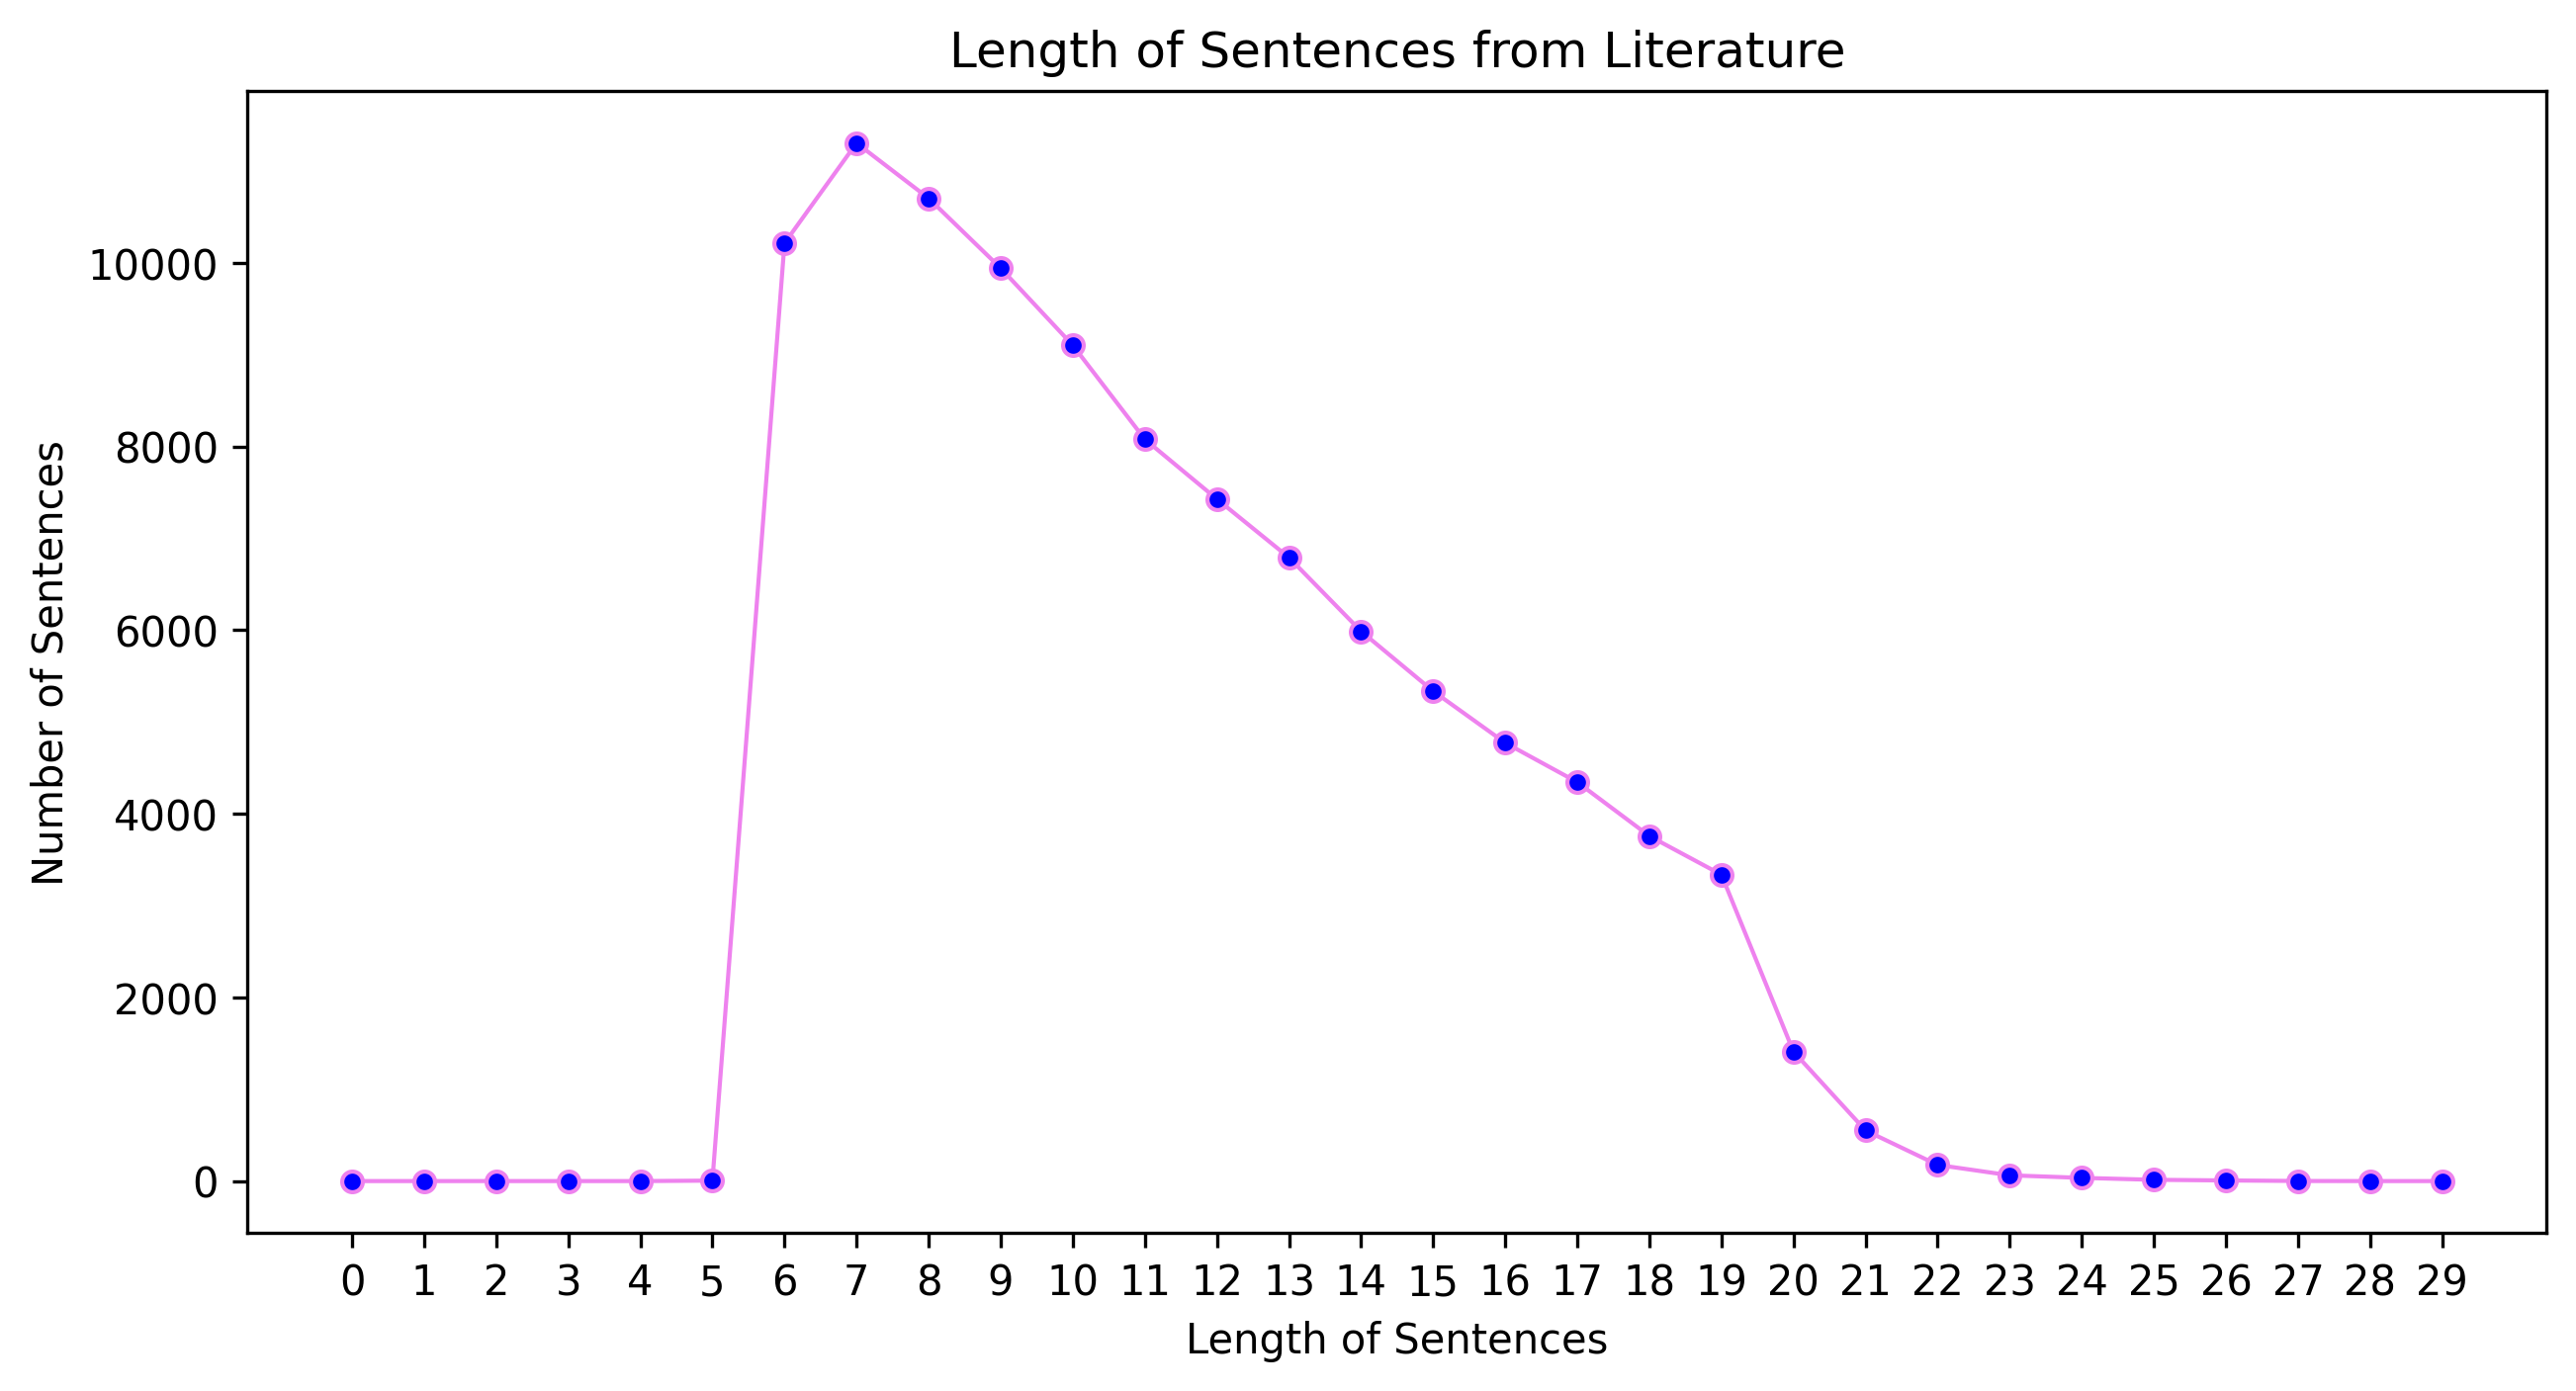
\includegraphics[scale=.7]{Images/Graph/output3.png}
                \caption{Number of words in Literature }
            \label{fig: Number of words in Literature}
        \end{figure}
        \newpage
        
        \begin{figure}[h!]
            \centering
            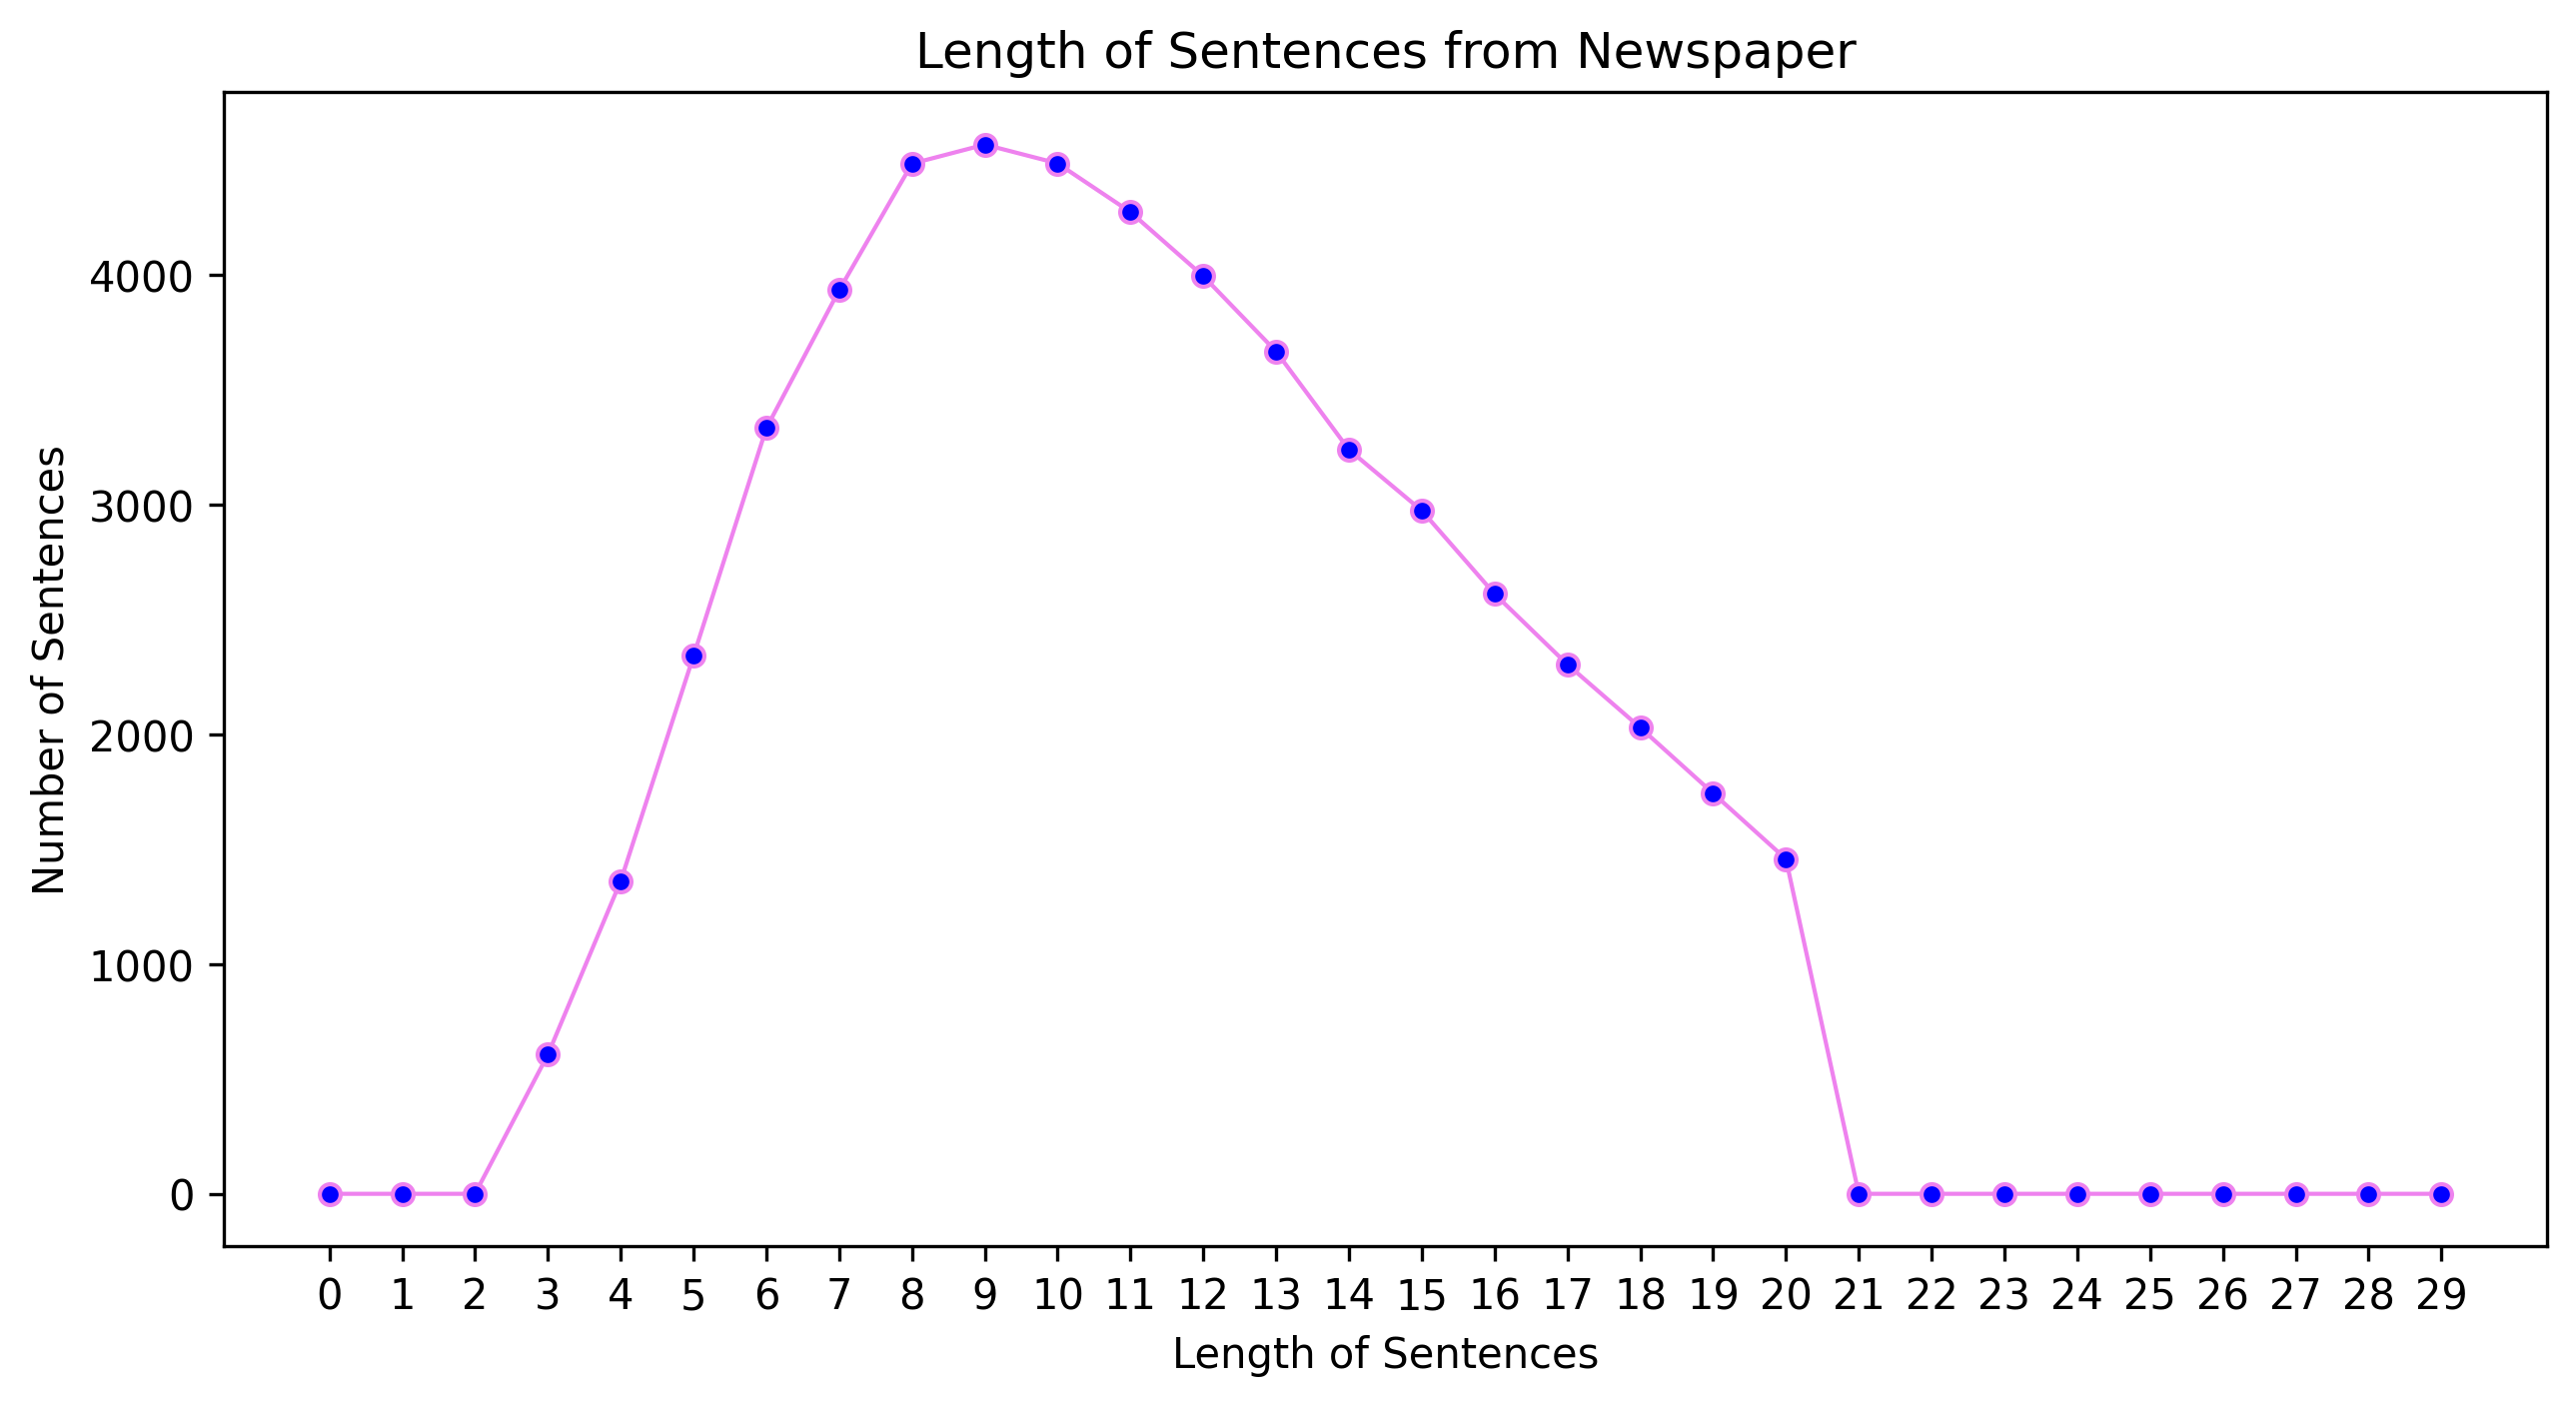
\includegraphics[scale=.7]{Images/Graph/output4.png}
                \caption{Number of words in Newspaper}
            \label{fig: Number of words in Newspaper}
        \end{figure}
        
                    \begin{figure}[h!]
            \centering
            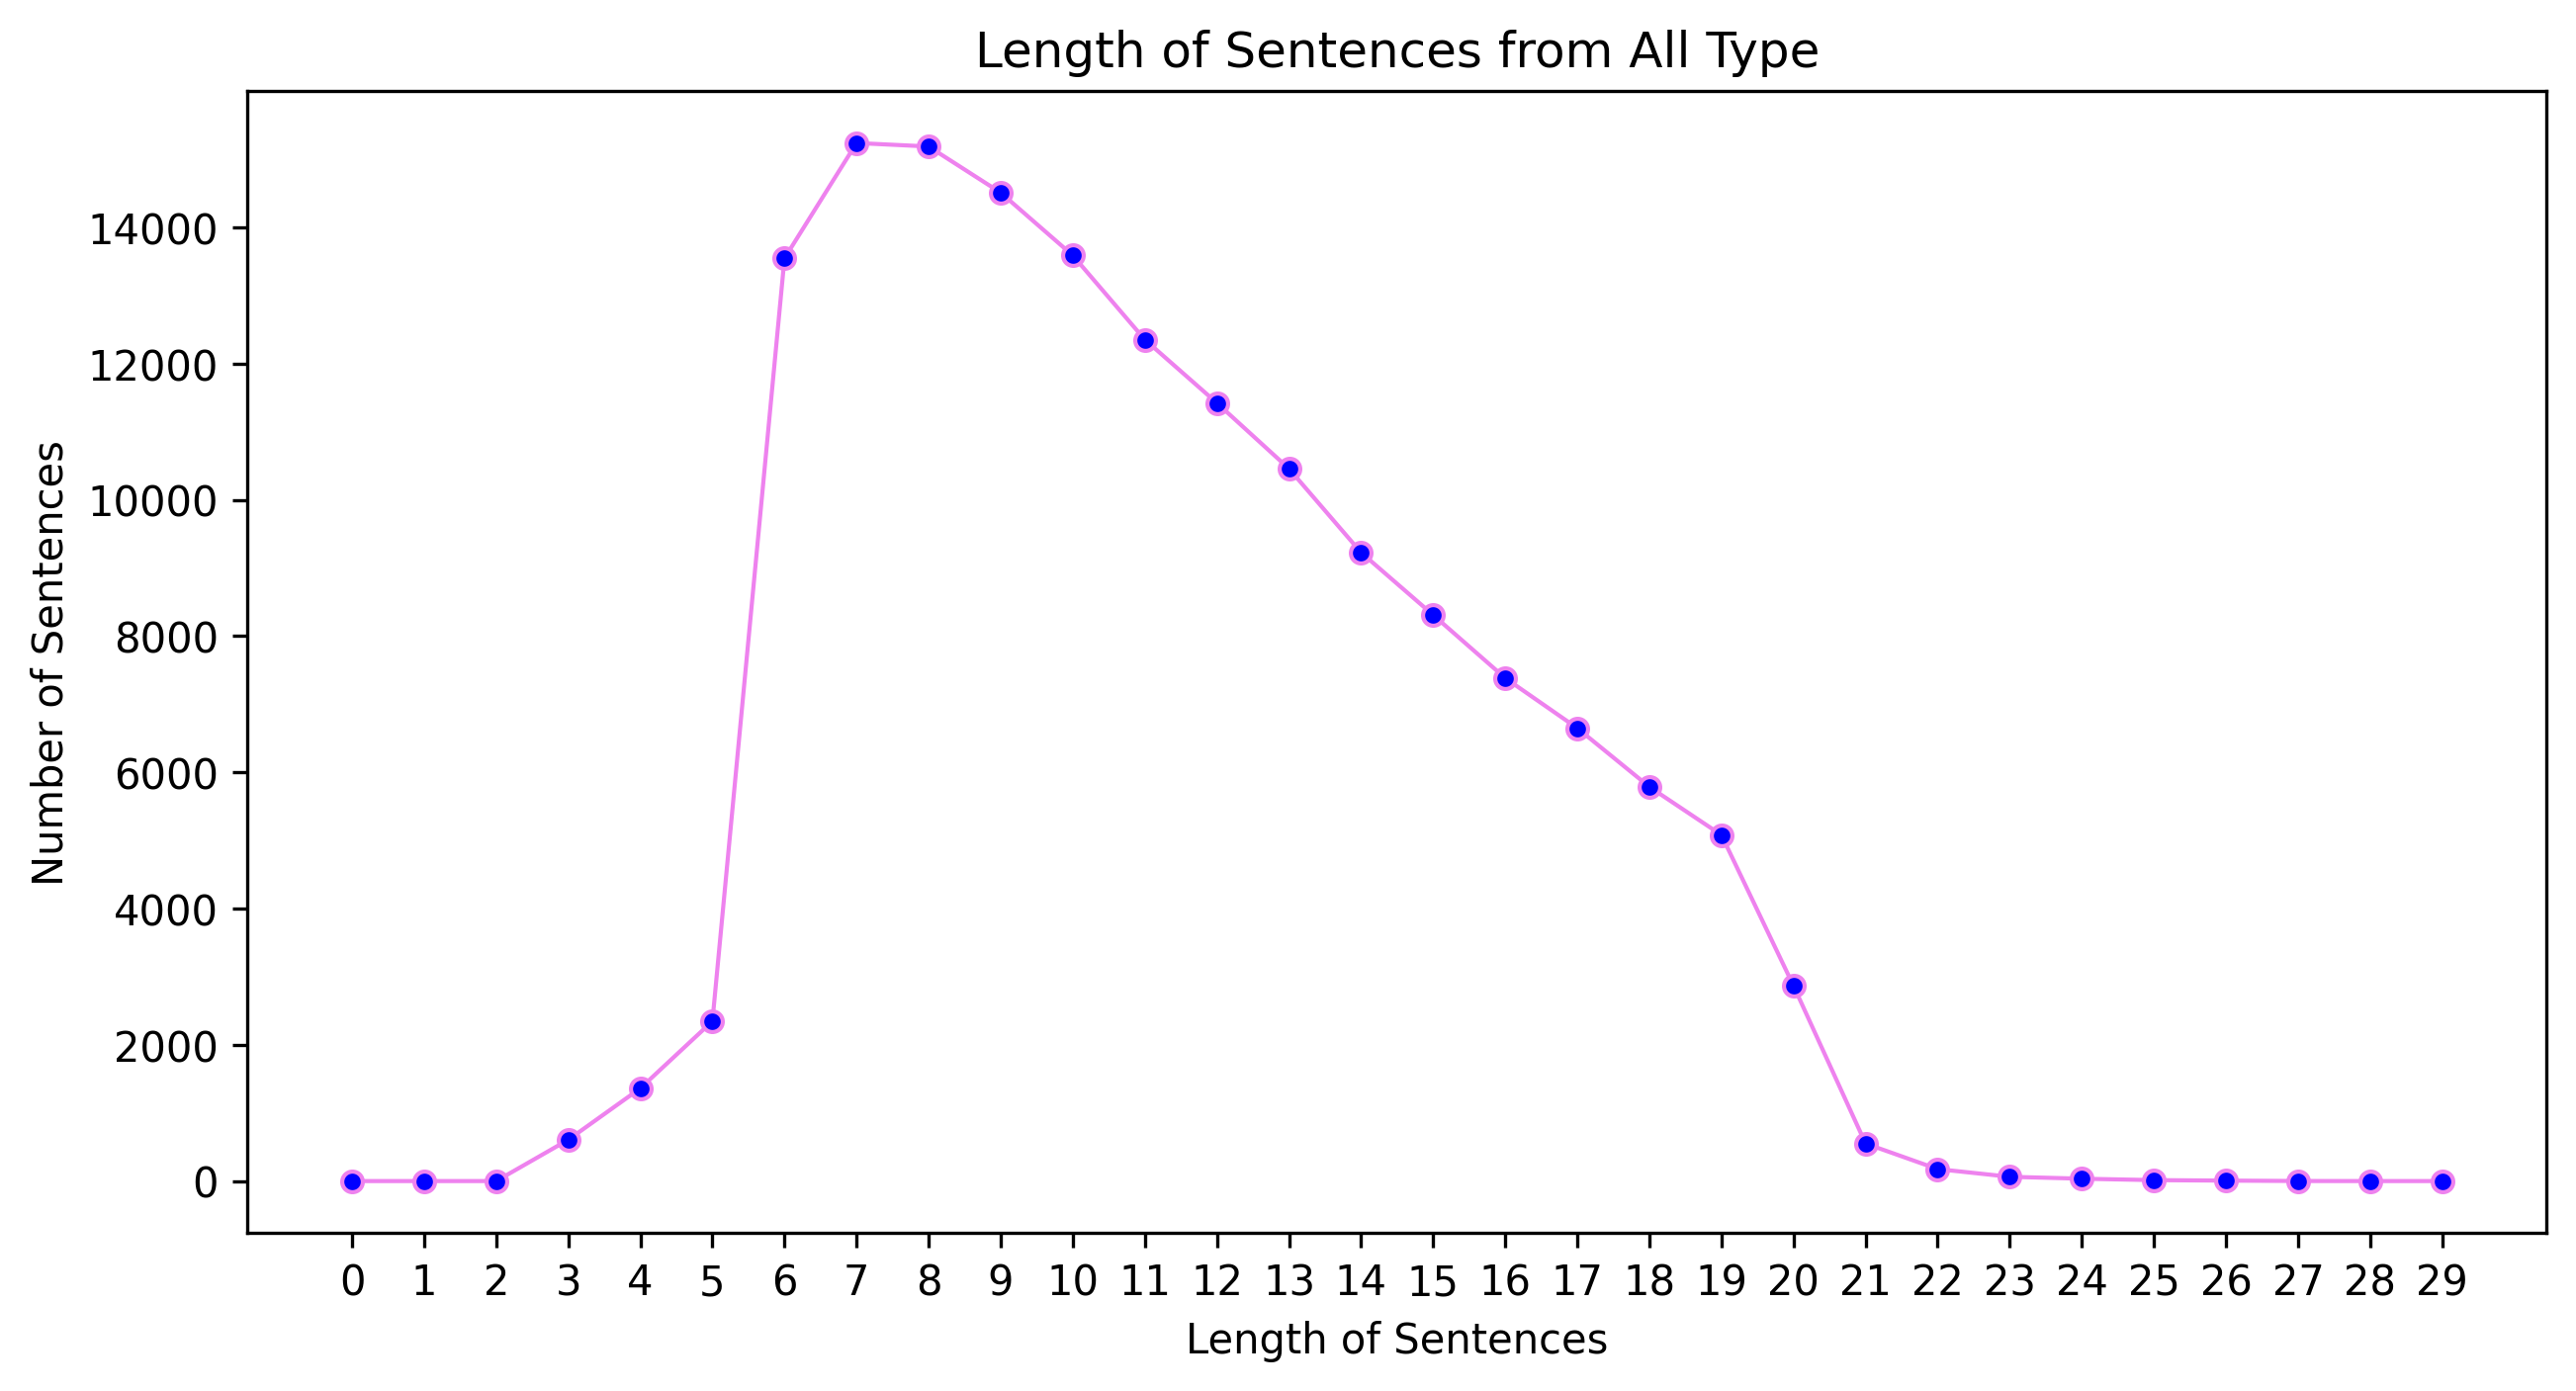
\includegraphics[scale=.7]{Images/Graph/output-all.png}
                \caption{Number of words in All Type}
            \label{fig: Number of words in All Type}
        \end{figure}

\subsection{Challenges in Sourcing}
As different platforms and formats have different data structures and most of them are not
in a standard format when scraped, we had to study the data types first properly in order
to find patterns so that we can maximize our output in terms of number and quality.

\section{Data Preparation}

\subsection{Cleaning}
\begin{itemize}
    \item As the word-level data was provided by Bengali.AI, it was already cleaned. So, we used it directly for transcription,
    \item On the other hand, the sentence-level data was fully sourced and curated by us from scratch. So, we had to programmatically and manually clean those from the dataset.
\end{itemize}

\section{IPA Transcription Process}

We were given a few words and IPA. We constructed a simple septa graph to identify unique phonemes. Using these phonemes and septa graph we made a Jupiter notebook that can generate IPA given a word. The notebook generates 116 IPAs.
        \begin{figure}[h!]
            \centering
            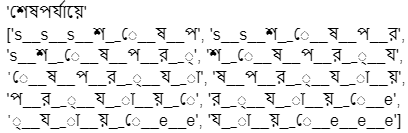
\includegraphics[scale=0.8]{Images/Screenshot/septa-graph.png}
                \caption{Septa graph}
            \label{fig: Septa graph}
        \end{figure}

\subsection{Word-Level Transcription Framework}
\begin{itemize}
    \item Using the notebook, we generated 56k IPAs for the 56k sentences provided to us by Bengali.AI which were taken from newspapers.
    \item These sentences had, 43356 unique words.
    \item We generated the IPAs for these words and gave them to the linguist team for initial validation.
    \item The linguist team validated these words and found some IPA mischaracterization, such as:\ipa{("a" , "ɐ"),("i" , "ɪ"),("æ" , "ɛ"),("r" , "ɾ"),("ʲ ","e̯ ")}
    \item Using these validated words and new characters, we fixed the 56k sentences and gave them to the linguist team for final word-level validation.
\end{itemize}
\newpage
\subsection{Sentence-Level Transcription Framework}

Process of replacing validated IPA words in generated IPA sentences.


First, we found the special characters in all sentences of the dataset.
%img
        \begin{figure}[h!]
            \centering
            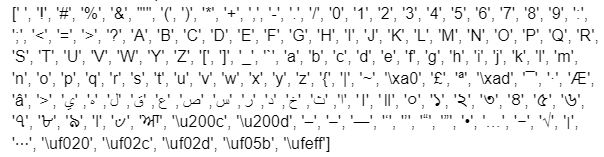
\includegraphics[scale=1]{Images/Screenshot/Special-char.png}
            \caption{Special Characters}
            \label{fig: Special Characters}
        \end{figure}

Then we concat all the sentences using the special character " \_\$\_ " .


%img
        \begin{figure}[h!]
            \centering
            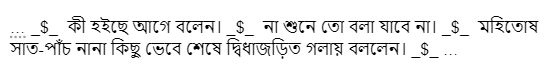
\includegraphics[scale=1]{Images/Screenshot/sentence-concat.png}
            \caption{Concated sentences}
            \label{fig: Concated sentences}
        \end{figure}
   
We identified the words and replaced them in place with the corresponding IPS.
Replaced words were marked with the prefix \_\_\#\#\_\_.

        \begin{figure}[h!]
            \centering
            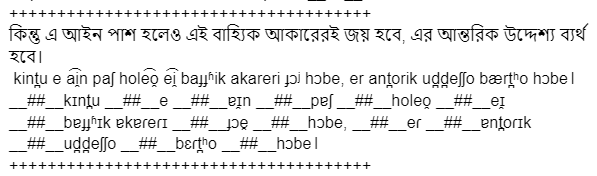
\includegraphics[scale=0.8]{Images/Screenshot/replace-word.png}
                \caption{Replaced words}
            \label{fig: Replaced words}
        \end{figure}
        

Then split the mixed sentence on " \_\$\_ ". So the IPA sentence Indexes matched the main index.

Then we found the IPA sentences that contained Bengali words and re-run the sentence with the notebook.

\newpage
\section{Validation}
A team of four individuals with undergraduate and graduate degrees
in linguistics in the supervision of Professor Dr. Syed Shahrier Rahman from the University of Dhaka was entrusted to do the annotation and validation of the whole DUAL-IPA dataset for every step.
\vspace{1cm}
 \begin{figure*}[htbp]
    \centering
    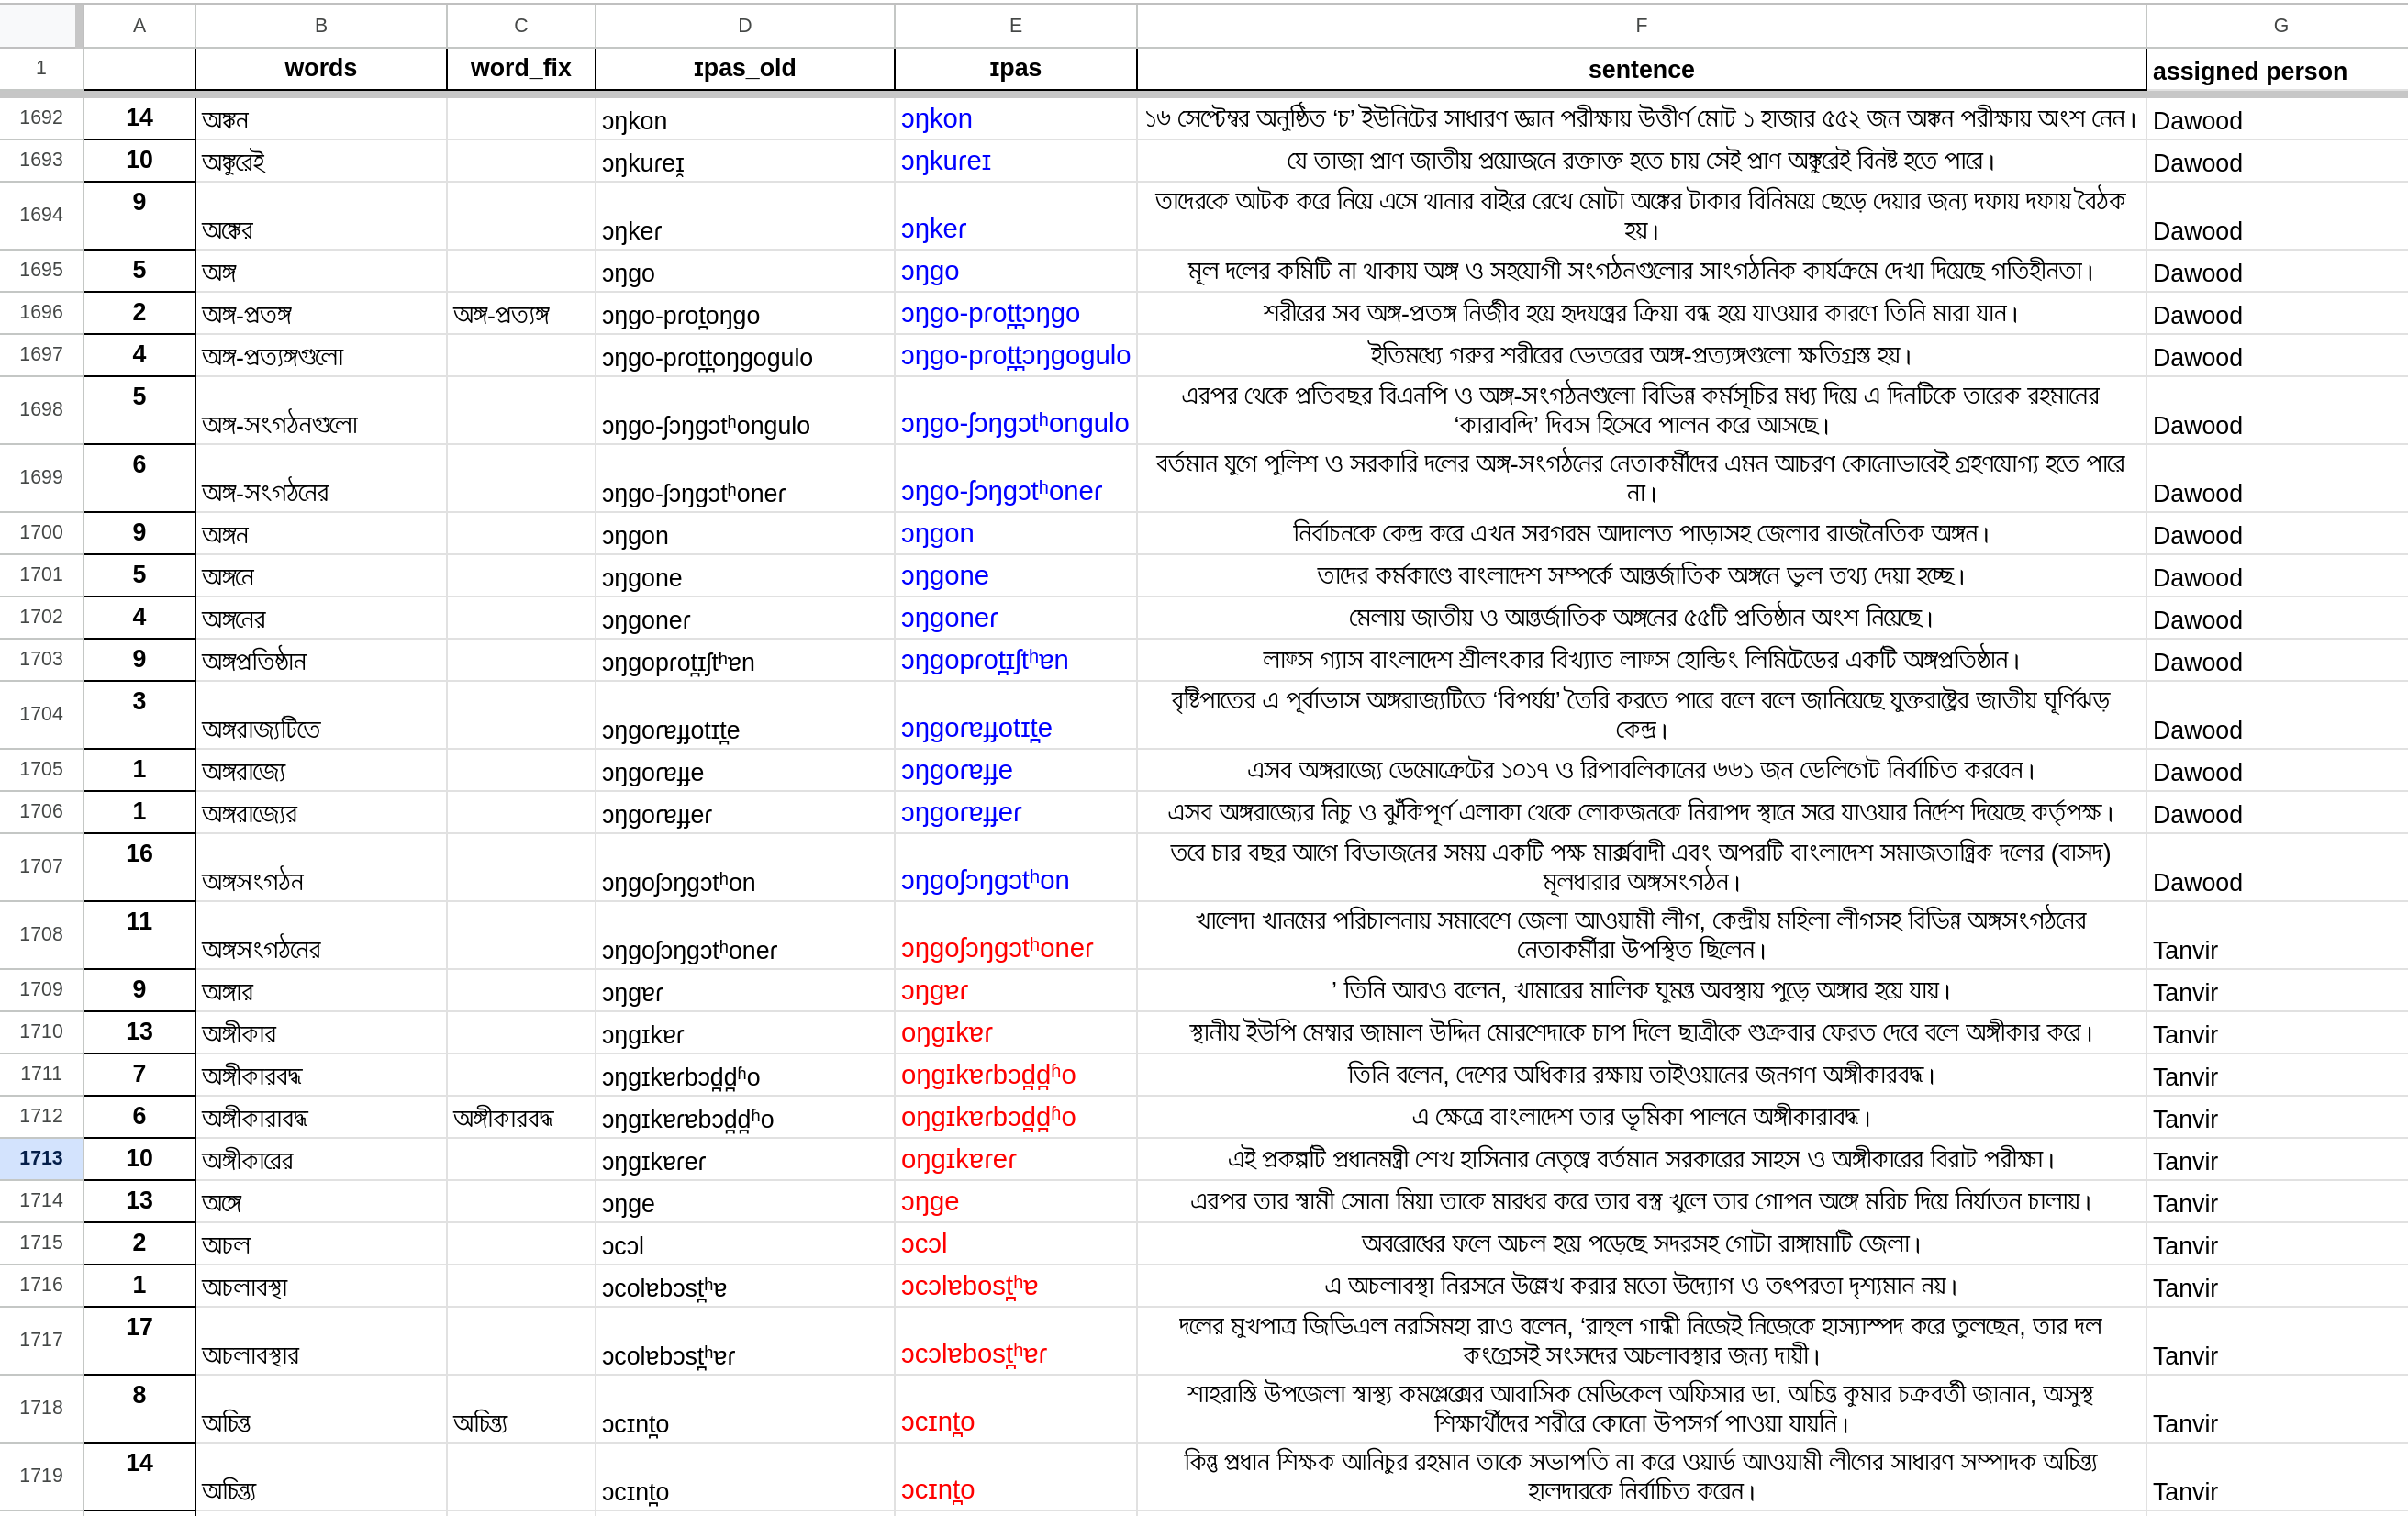
\includegraphics[width=\textwidth]{Images/Screenshot/unique_words.png}
    \caption{Validation stage of the linguistics team}
    \label{fig:unique_words}
\end{figure*} 



\subsection{Metrics}
Linguists made sure to follow all the latest Bangla Academy conventions for spelling and pronunciation of the words that are included in the dataset, as well as they made sure to follow all the standards of the IPA conventions in the whole process. The dataset had to go through multiple validation steps. Each step made sure to increase the quality of this work.
\newpage
\subsection{Results}
With the help of the linguists team, the final output which is the preparation of DUAL-IPA dataset was possible with the highest level of accuracy from our end. Here is figure \ref{fig:types} showing Number and Types of Words in Dataset.

 \begin{figure*}[htbp]
    \centering
    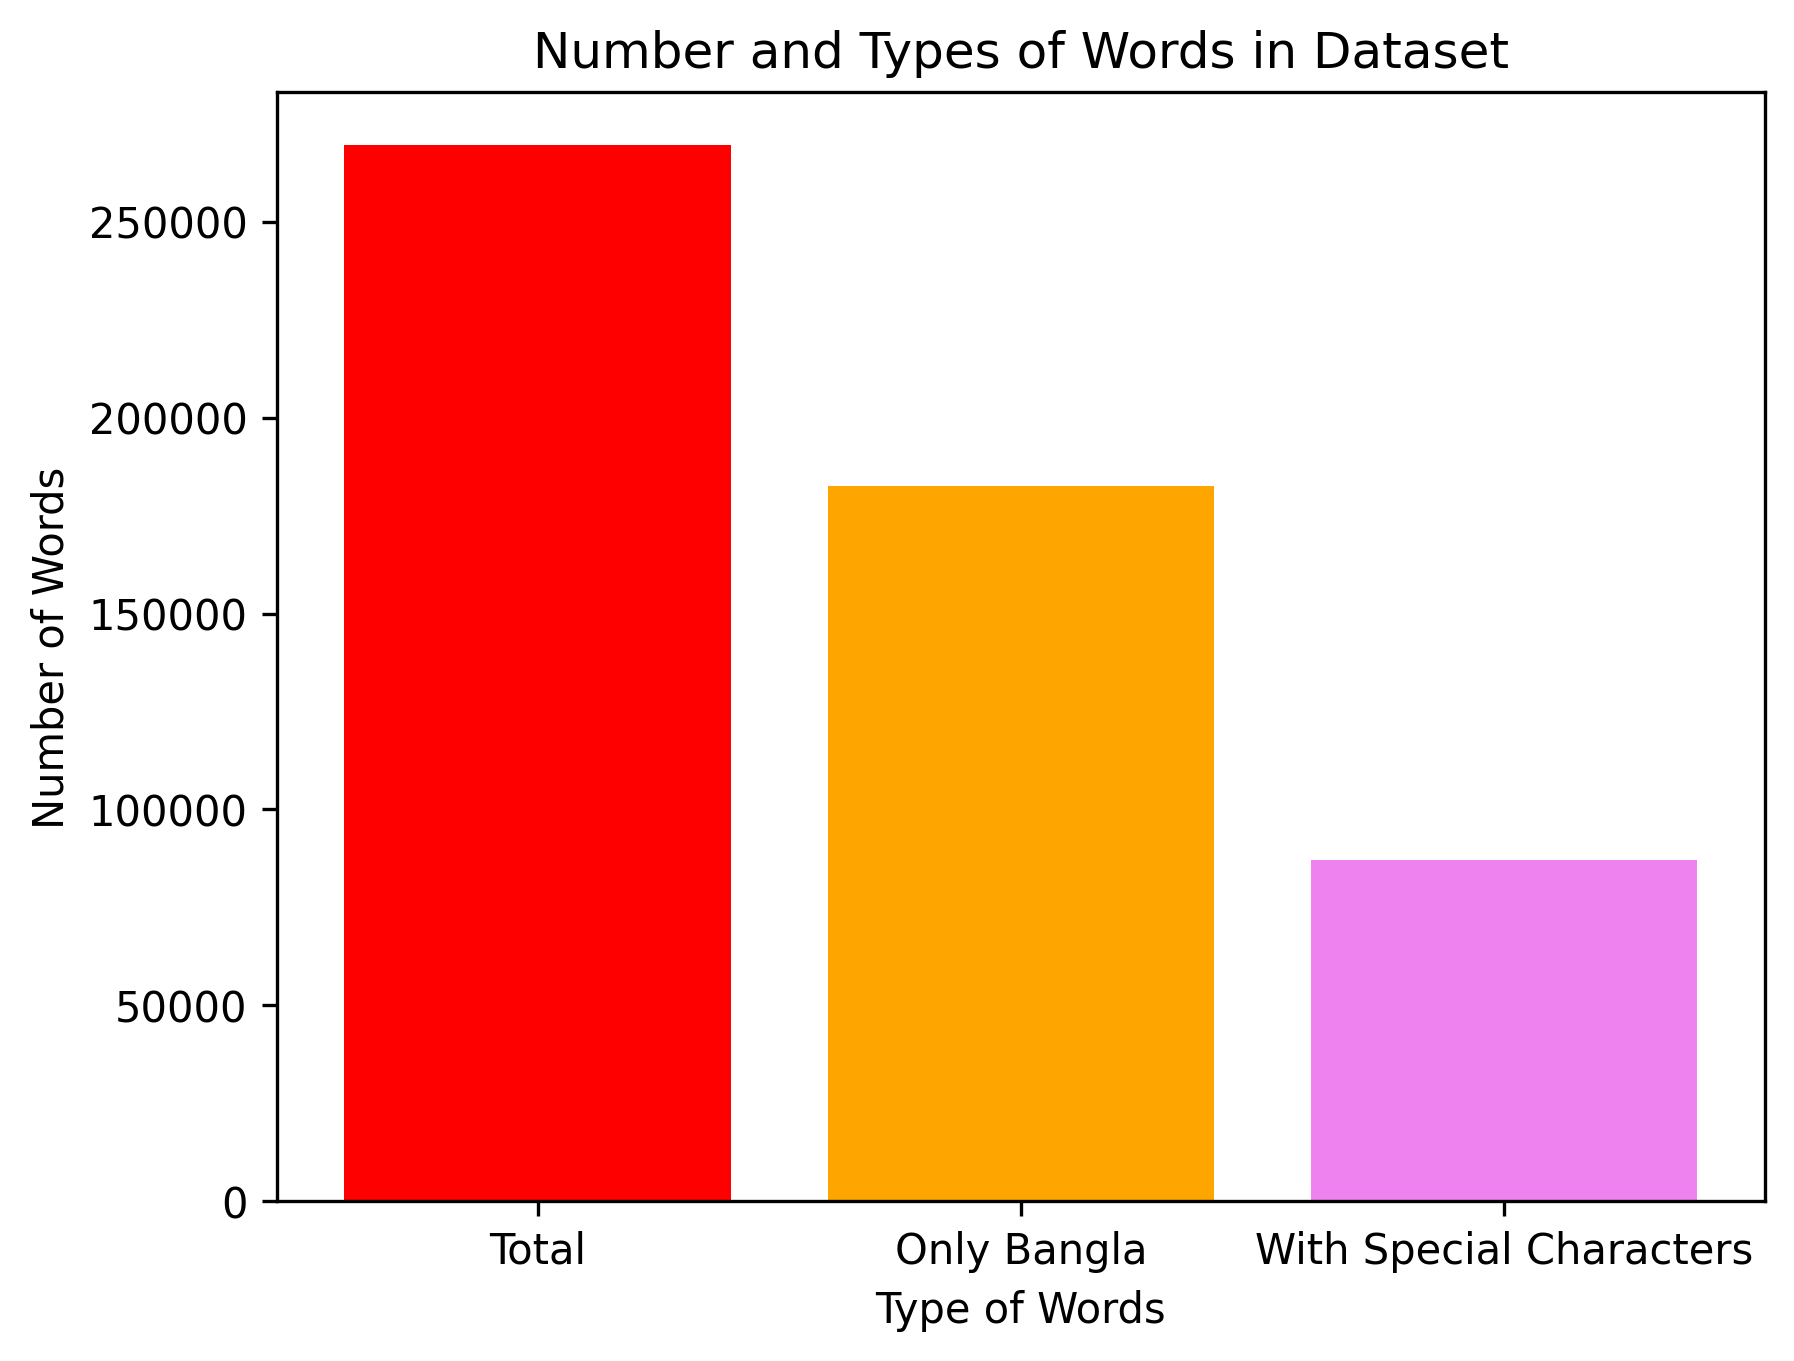
\includegraphics[width=\textwidth]{Images/Graph/output1.png}
    \caption{Number and Types of Words in Dataset}
    \label{fig:types}
\end{figure*} 

\newpage
\section{Ethical Considerations}

\subsection{Privacy:} No personally identifiable information (PII) was directly collected or stored within the dataset. All the data are collected from public sources only.

\subsection{Bias:} As the dataset comprises text scraped from online sources, it may inadvertently reflect potential biases present in the original content. We acknowledge this inherent limitation and emphasize the importance of using the dataset responsibly and considering potential biases during analysis and interpretation of results. Additionally, we encourage further research into developing debiasing techniques for NLP applications using such datasets.

\subsection{Transparency:} We have documented the data collection process and annotation guidelines with transparency, enabling users to understand the potential limitations and biases associated with the dataset. Sharing this information encourages responsible use and facilitates further discussion about ethical considerations in NLP research.

\subsection{Respect:} Throughout the research process, we maintained respect for the cultural and linguistic nuances of the Bangla language. We consulted with language experts and adhered to established IPA transcription protocols to ensure the accuracy and cultural sensitivity of the dataset.

By acknowledging and addressing these ethical considerations, we strive to promote responsible development and utilization of the DUAL-IPA dataset, contributing to ethical advancements in Bangla NLP research.